\documentclass{article}

\usepackage{hyperref}
\usepackage{nomencl}
\usepackage{blkarray} % customed arrays
\usepackage{amsmath} % matrix equations
\usepackage{graphicx} % import images
\usepackage{float} % floating imgs
\usepackage{subcaption} % several figures on one line
\graphicspath{ {ressources/} }
\makeglossary

\title{Computational Methods \& C++ Assignment}
\author{Augustin Reille}
\date{2 November 2017}

\begin{document}
    % Title
    \maketitle

    % Abstract
    \begin{abstract}
        A one-space dimensional problem is considered, to examine the application
        of numerical schemes for the solution of partial differential equations. 
    \end{abstract}

    % Table of contents
    \newpage
    \tableofcontents

    % List of figures
    \newpage
    \listoffigures

    % List of tables
    \listoftables

    % List of abbreviations / Nomenclature
    

    % Introduction
    \newpage
    \section{Introduction}

    
    % Methods / Procedures
    \newpage
    \section{Methods}


        Several methods are used :
        \begin{itemize}
            \item{Dufort-Frankel}
            \item{Richardson}
            \item{Laasonen simple implicit}
            \item{Crank-Nicholson}
        \end{itemize}
        For all of the used schemes, the initialization of the result matrix is run the same way.
        First the study grid must be chosen. The initials conditions are:
        \begin{itemize}
            \item{$T_{int}$ of 100$^{\circ}$F}
            \item{$T_{sur}$ of 300$^{\circ}$F}
            \item{$D = 0.1 ft^{2}/hr$}
        \end{itemize}
        First it was assumed that $\Delta x = 0.05$ and $\Delta t = 0.01$,
        so that the result matrix could be initialized.
        We set:
        \begin{equation}
            n_{space} = \frac{L}{\Delta x} + 1
        \end{equation}
        \begin{equation}
            n_{time} = \frac{T}{\Delta t}
        \end{equation}
        $n_{space}$ is the number of iterations over the grid, according to the coordinate $x$. \\
        $n_{time}$ is the number of iterations over the grid, according to the time $t$. \\
        
        \[
            \begin{blockarray}{cccccc}
            i=0 & i=1 & \cdots & n_{space}-1 & n_{space} \\
            \begin{block}{(ccccc)c}
              T_{ext} & T_{int} & \cdots & T_{int} & T_{ext} & j=0 \\
              T_{ext} & 0 & \cdots & 0 & T_{ext} & j=1 \\
              \vdots & \vdots & \ddots & \vdots & \vdots & \vdots \\
              T_{ext} & 0 & \cdots & 0 & T_{ext} & n_{time} \\
            \end{block}
            \end{blockarray}
        \]
        This is how the matrix is initialized, according to initial conditions.
        For most of the used schemes, we need two previous time steps to calculate the current step.
        An order one scheme (FTCS) is used to find the second line of the matrix:
        \begin{equation}
            T_{i,1} = \frac{\alpha}{2} (T_{i+1,0} + T_{i-1,0}) + (1-\alpha)T_{i,0}
        \end{equation}
        with $$\alpha = 2\frac{D\delta t}{\delta x^{2}}$$
        So we have:
        \[
            \begin{blockarray}{cccccc}
            i = 0 & i = 1 & \cdots & n_{space}-1 & n_{space} \\
            \begin{block}{(ccccc)c}
              T_{ext} & T_{int} & \cdots & T_{int} & T_{ext} & j=0 \\
              T_{ext} & T_{i,1} & \cdots & T_{i,1} & T_{ext} & j=1 \\
              \vdots & \vdots & \ddots & \vdots & \vdots & \vdots \\
              T_{ext} & 0 & \cdots & 0 & T_{ext} & n_{time} \\
            \end{block}
            \end{blockarray}
        \]
        With this trick our matrix is ready to be used and filled up with every scheme.

        \subsection{Explicit schemes}
            For both of the explicit schemes used (Dufort-Frankel and Richardson schemes), the solving
            is run the same way : with a double for-loop, the matrix is filled up. The only thing that change
            is the way we advance through time and space.

            \subsubsection{Dufort-Frankel}
                Explicitly, for Dufort-Frankel method, we have:
                \begin{equation}
                    \label{eq:df}
                    T_{j}^{n+1} = (\frac{1-\alpha}{1+\alpha})T_{j}^{n-1} + (\frac{\alpha}{1+\alpha})(T_{j+1}^{n}+T_{j-1}^{n})
                \end{equation}
                with $$\alpha = 2\frac{D\delta t}{\delta x^{2}}$$

            \subsubsection{Richardson}
                Explicitly, for Richardson method, we have:
                \begin{equation}
                    \label{eq:rich}
                    T_{j}^{n+1} = T_{j}^{n-1} + \alpha (T_{j-1}^{n} - 2T_{j}^{n} + T_{j+1}^{n})
                \end{equation}
                with $$\alpha = 2\frac{D\delta t}{\delta x^{2}}$$

        \subsection{Implicit schemes}

                For both implicit schemes, the vector solution is given by a matrix equation. A $LU$
                factorization is used once, before a for-loop, to resolve the system for each space step.

                \subsubsection{Laasonen}

                We have :
                \begin{equation}
                    \frac{T_{j}^{n+1} - T_{j}^n}{\Delta t} = D \frac{T_{j+1}^{n+1}- 2T_{j}^{n+1} + T_{j-1}^{n+1}}{\Delta x^2}
                \end{equation}

                Written in a matrical way, the solution at space step $n+1$ is given by :
                \begin{equation}
                    \begin{bmatrix}
                        1+2C   & -C     & 0      & \cdots & 0 \\
                        -C     & 1+2C   & -C     & \ddots & \vdots \\
                        0      & -C     & \ddots & \ddots & 0 \\
                        \vdots & \ddots & \ddots & 1+2C   & -C\\
                        0      & \cdots & 0      & -C     & 1+2C
                    \end{bmatrix}
                    \begin{bmatrix}
                        T_{1} \\
                        T_{2} \\
                        \vdots \\
                        T_{i} \\
                        \vdots \\
                        T_{ntime}
                    \end{bmatrix}_{n+1}
                    =
                    \begin{bmatrix}
                        T_{1} + CT_{0}\\
                        T_{2} \\
                        \vdots \\
                        T_{i} \\
                        \vdots \\
                        T_{ntime} + CT_{f}
                    \end{bmatrix}_{n}
                \end{equation}
                with $$C = \frac{D\Delta t}{\Delta x ^2}  $$ 
                The first vector at space $n$ is our boundaries conditions vector, so it is known.
                In this scheme we must be aware that the right-term vector is actually bigger than
                the other, of 2 values, which corresponds to the exterior temperatures, which stays
                the same all the time.\\
                We apply the $LU$ solve algorithm for each space step, at the reduced vector, and add the $n+1$ vector to our 
                result matrix. The new right term vector is the one found with the $LU$ solve algorithm.
 
                \subsubsection{Crank-Nicholson}
                    We have :
                    \begin{equation}
                        \frac{T_{j}^{n+1} - T_{j}^n}{\Delta t} = D\frac{1}{2} (\frac{T_{j+1}^{n+1}- 2T_{j}^{n+1} + T_{j-1}^{n+1}}{\Delta x^2}+\frac{T_{j+1}^{n}- 2T_{j}^{n} + T_{j-1}^{n}}{\Delta x^2})
                    \end{equation}
                    Written in a matrical way, the solution at space step $n+1$ is given by :
                    \begin{equation}
                        \begin{bmatrix}
                            1+C    & -C/2   & 0     & \cdots & 0 \\
                            -C/2   & 1+C    & -C/2   & \ddots & \vdots \\
                            0      & -C/2   & \ddots & \ddots & 0 \\
                            \vdots & \ddots & \ddots & 1+C   & -C/2\\
                            0      & \cdots & 0      & -C/2   & 1+C
                        \end{bmatrix}
                        \begin{bmatrix}
                            T_{1} \\
                            T_{2} \\
                            \vdots \\
                            T_{i} \\
                            \vdots \\
                            T_{ntime}
                        \end{bmatrix}_{n+1}
                    \end{equation}
                    \[
                        =
                        \begin{bmatrix}
                            1-C    &C/2    & 0      & \cdots & 0 \\
                            C/2     & 1-C   & C/2     & \ddots & \vdots \\
                            0      & C/2     & \ddots & \ddots & 0 \\
                            \vdots & \ddots & \ddots & 1-C   & C/2\\
                            0      & \cdots & 0      & C/2     & 1-C
                        \end{bmatrix}
                        \begin{bmatrix}
                            T_{1} + CT_{0}\\
                            T_{2} \\
                            \vdots \\
                            T_{i} \\
                            \vdots \\
                            T_{ntime} + CT_{f}
                        \end{bmatrix}_{n}
                    \]
                    with $$C = \frac{D\Delta t}{\Delta x ^2}  $$ 
                    The method is the same as Laasonen scheme, except that the left term vector found with the $LU$ solve
                    algorithm is multiplied by the right term matrix before the next space step.

            \subsection{Analytical solution}
                The analytical solution of the problem considered will be used to compare our results and to calculate
            the errors. The result of the analytical solution for a time $t$ and a position $x$ is given by : 
            \begin{equation}
                \label{eq:analytical}
                T = T_{ext}+2(T_{int}-T_{ext})\sum_{m=1}^{m=\infty} e^{-D(m\pi / L)^{2}t} \frac{1-(-1)^m}{m\pi} sin(\frac{m\pi x}{L})
            \end{equation}


            \subsection{Object Oriented Design}

            The object oriented classes for the C++ code are designed the following way :\\
            \begin{figure}[H]
                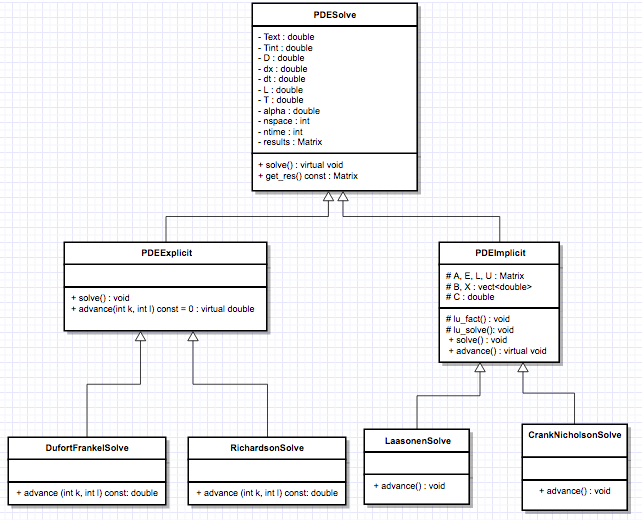
\includegraphics[width=\textwidth]{UML.png}
                \caption{UML Diagram of the C++ object oriented code}
            \end{figure}
            There is a main base class called PDESolve, which initializes all the variables, and two functions :
            \begin{itemize}
                \item{get\_res() : returns the results Matrix}
                \item{solve() : virtual function which will be overwritten in subclasses}
            \end{itemize}
            There is two subclasses of PDESolve : PDEExplicit and PDEImplicit. Each one has a solve() function, and a virtual advance function,
            which corresponds at the way the space and time steps are incrementded.
            The PDEImplicit class also initializes all the matrixes and functions needed for the LU factorization and solve.
            Each subsubclass, which corresponds to each method, has its own particular advance method.
    % Results
    \newpage
    \section{Results}
        \subsection{Schemes study}
            Note that results from Richardson scheme are not displayed on the following plots, due to its unstability \cite{rich}: 
        the incorrect values polluted our charts.
        \begin{figure}[H]
            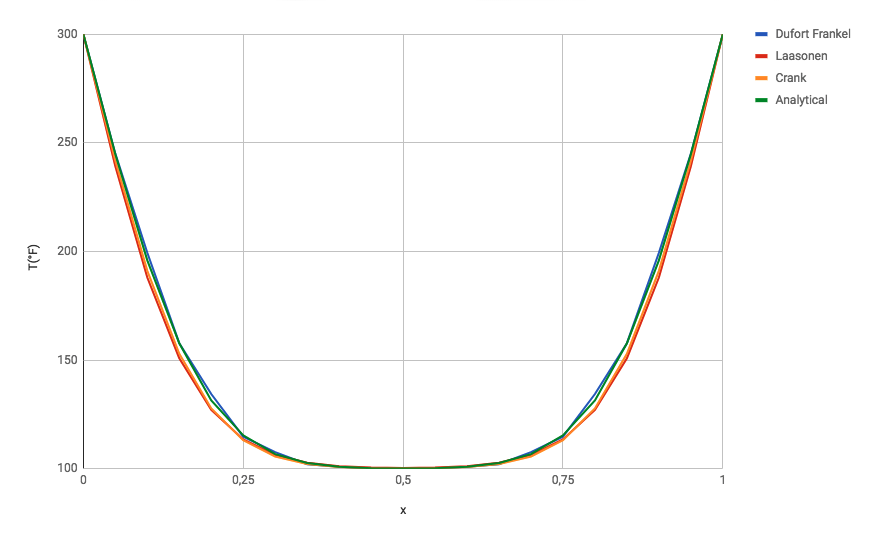
\includegraphics[width=\textwidth]{t01.png}
            \caption{Results with differents schemes at t = 0,1h}
        \end{figure}
        We can see that except for the Richardson scheme, the results are quite the same. The errors had been calculated 
        to evaluate the accuracy of each method.
        \begin{table}[H]
            \centering
            \caption{Errors for different schemes at t = 0,1h}
            \begin{tabular}{|c|c|c|c|l}
            \cline{1-4}
            Errors & Dufort-Frankel & Laasonen & Crank-Nicholson &  \\ \cline{1-4}
            1-norm & 0,56\%         & 1,72\%   & 1,26\%          &  \\ \cline{1-4}
            \end{tabular}
        \end{table}
        We observe that Dufort-Frankel method is the most accurate, 
        followed by the Crank-Nicholson method then by the Laasonen method. Let see the evolution of the error
        while time is increased.
        % \begin{figure}[H]
        %     \centering
        %     \begin{subfigure}[b]{0.45\textwidth}
        %         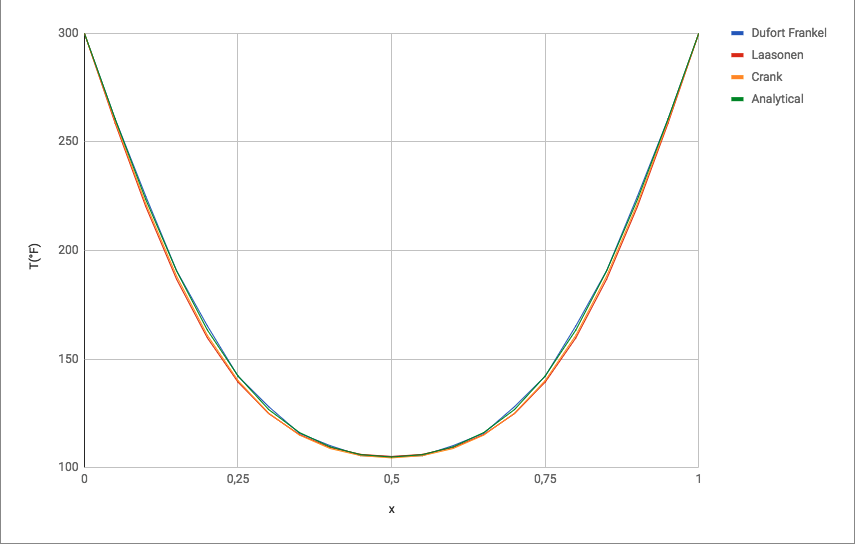
\includegraphics[width=\textwidth]{t02.png}
        %         \caption{t = 0,2h}
        %     \end{subfigure}
        %     \begin{subfigure}[b]{0.45\textwidth}
        %         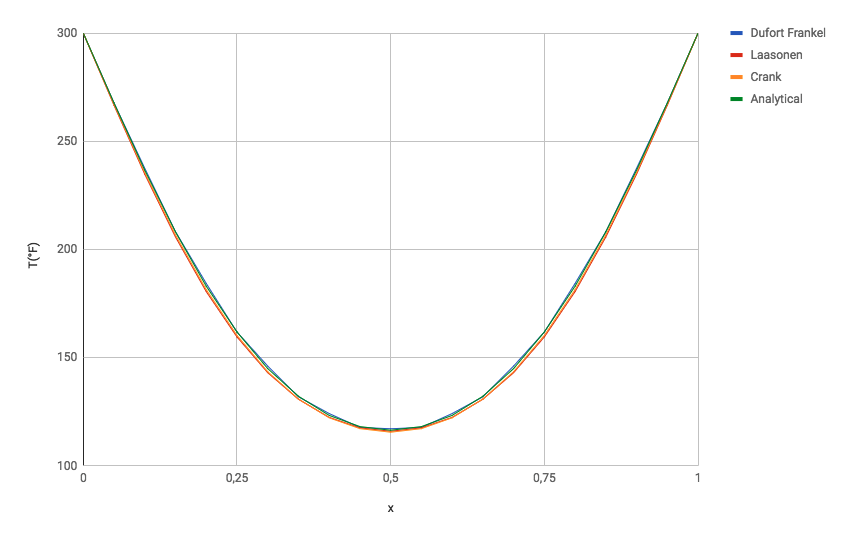
\includegraphics[width=\textwidth]{t03.png}
        %         \caption{t = 0,3h}
        %     \end{subfigure}
        %     \\
        %     \begin{subfigure}[b]{0.45\textwidth}
        %         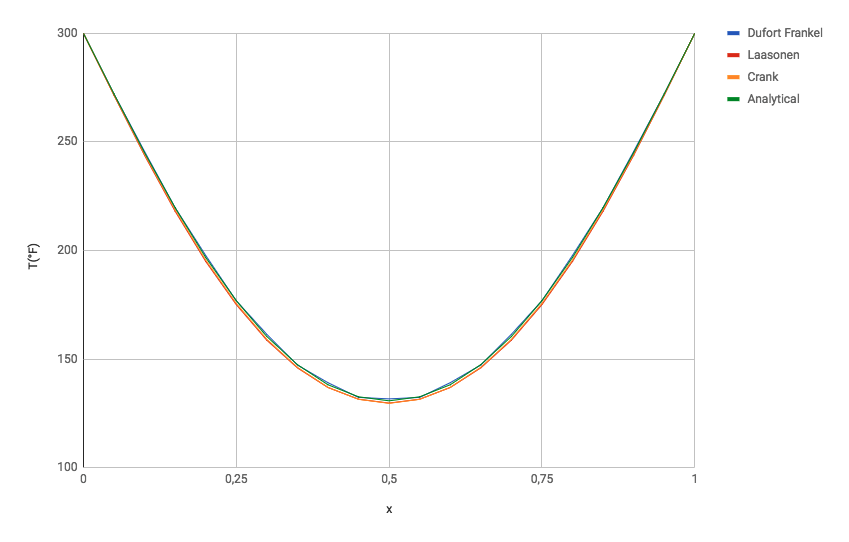
\includegraphics[width=\textwidth]{t04.png}
        %         \caption{t = 0,4h}
        %     \end{subfigure}
        %     \begin{subfigure}[b]{0.45\textwidth}
        %         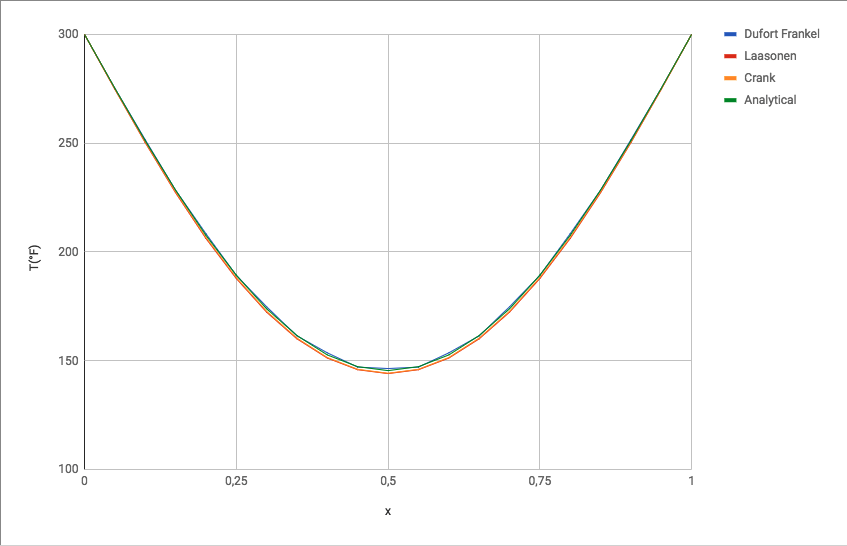
\includegraphics[width=\textwidth]{t05.png}
        %         \caption{t = 0,5h}
        %     \end{subfigure}
        %     \caption{Results with differents schemes at different times}
        % \end{figure}
        \begin{table}[H]
            \centering
            \caption{Errors for different schemes at different times}
            \begin{tabular}{|c|c|c|c|}
            \hline
            Errors & Dufort frankel & Laasonen & Crank-Nicholson \\ \hline
            t=0,2h & 0,37\%         & 1,05\%   & 0,80\%          \\ \hline
            t=0,3h & 0,27\%         & 0,77\%   & 0,60\%          \\ \hline
            t=0,4h & 0,22\%         & 0,64\%   & 0,49\%          \\ \hline
            t=0,5h & 0,18\%         & 0,55\%   & 0,42\%          \\ \hline
            \end{tabular}
        \end{table}

        We observe that the error is globally decreasing as time increase. The most accurate method appears to 
        be the Dufort-Frankel method, then the Crank-Nicholson method, then the Laasonen method.

        \subsection{Laasonen method : effect of the step time}
        \begin{figure}[H]
            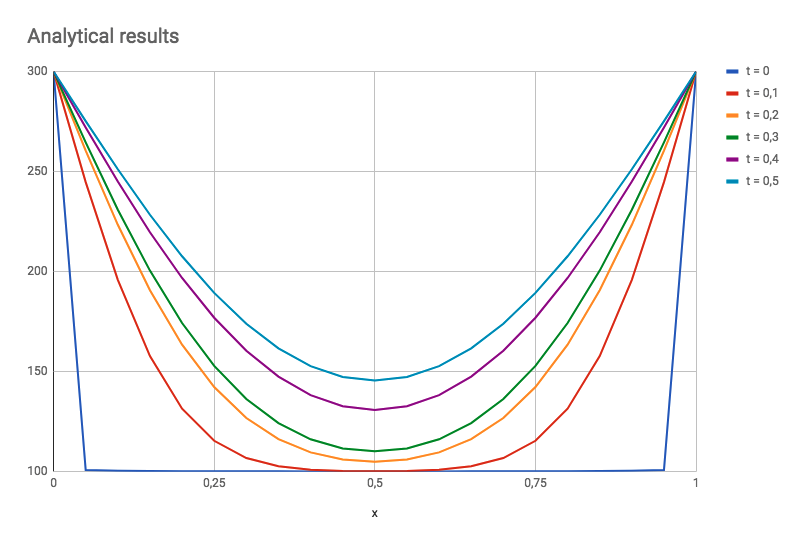
\includegraphics[width=\textwidth]{analytical.png}
            \caption{Analytical results at different times}
        \end{figure}
        % \begin{figure}[H]
        %     \centering
        %     \begin{subfigure}[b]{0.45\textwidth}
        %         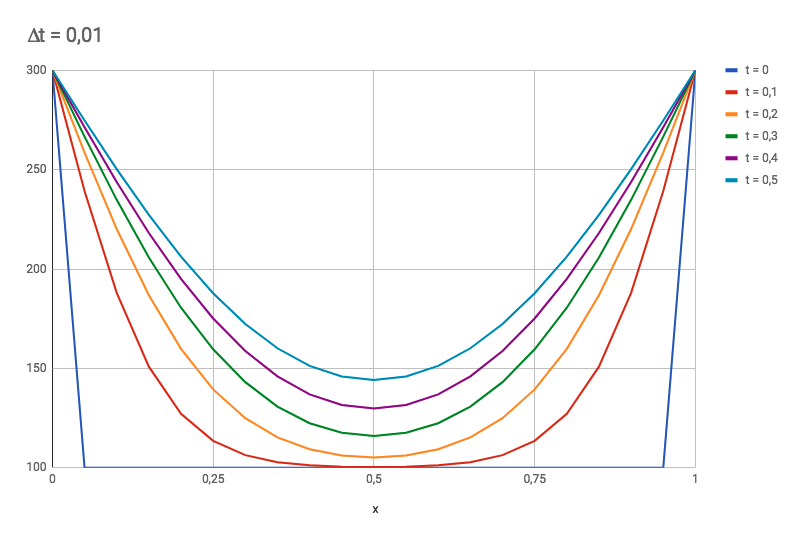
\includegraphics[width=\textwidth]{las-1.png}
        %         \caption{$\Delta t$ = 0,01}
        %     \end{subfigure}
        %     \begin{subfigure}[b]{0.45\textwidth}
        %         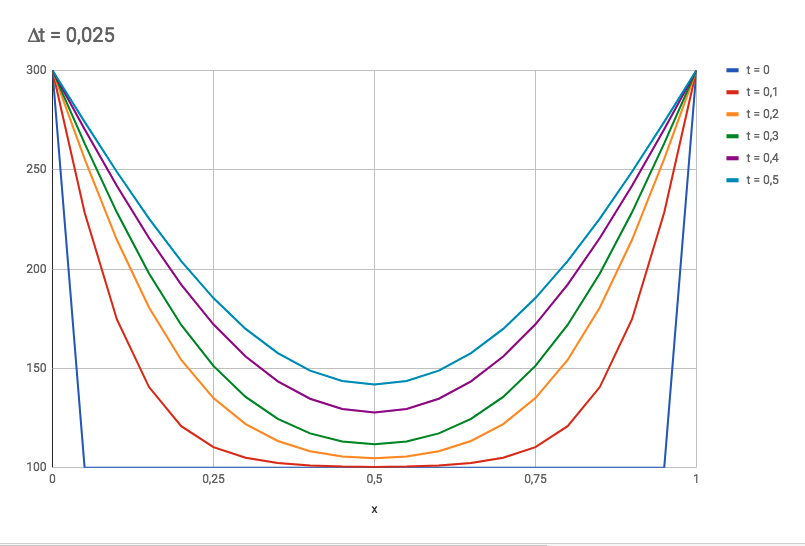
\includegraphics[width=\textwidth]{las-2.png}
        %         \caption{$\Delta t$ = 0,025}
        %     \end{subfigure}
        %     \\
        %     \begin{subfigure}[b]{0.45\textwidth}
        %         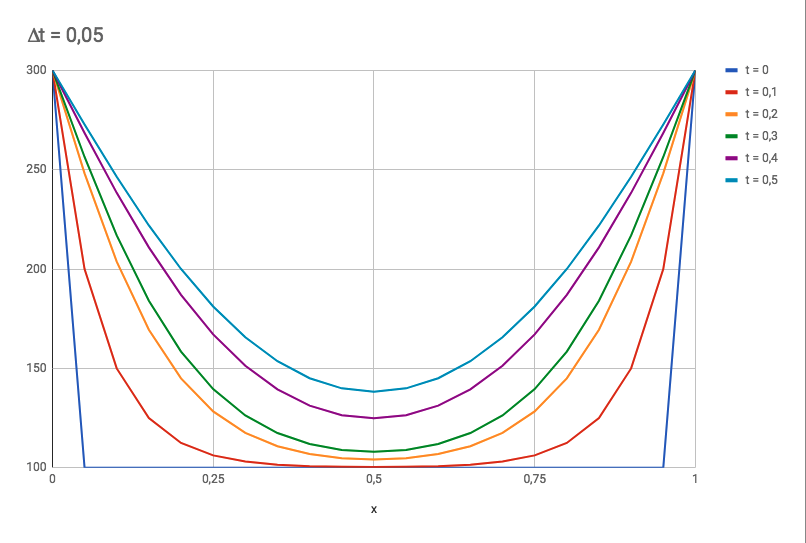
\includegraphics[width=\textwidth]{las-3.png}
        %         \caption{$\Delta t$ = 0,05}
        %     \end{subfigure}
        %     \caption{Effect of time step increasing on Laasonen scheme}
        % \end{figure}
        We can see that the shape of the results is more accurate as $\Delta t$ is little.
        It may be assumed that increasing $\Delta t$ gives less accurate results.
        Let's calculate the error between these values and the analytical values.

        \begin{table}[H]
            \centering
            \caption{Laasonen - effect of time step increasing }
            \label{table:laas}
            \begin{tabular}{|l|l|l|l|l|l|}
                \hline
                Errors    & t = 0,1h & t = 0,2h  & t = 0,3h  & t = 0,4h & t = 0,5h \\ \hline
                $\Delta$t=0,01  & 1,72\%   & 1,05\%  & 2,83\%  & 0,64\% & 0,55\% \\ \hline
                $\Delta$t=0,025 & 4,53\%   & 2,76\%  & 0,81\%  & 1,69\% & 1,45\% \\ \hline
                $\Delta$t=0,05  & 9,75\%   & 5,84\%  & 4,95\%  & 3,50\% & 2,98\% \\ \hline
                $\Delta$t=0,1   & 53,96\%  & 12,80\% & 16,30\% & 7,35\% & 6,19\% \\ \hline
            \end{tabular}
        \end{table}

        We observe that as time grows, the error decrease. Also, as time step grows, the error is increasing.
        Previous asumption is correct, according to the error calculation.
    % Discussion
    \newpage
    \section{Discussion}
        \subsection{Analytical solution}
            First thing that should be considered is that the analytical solution should not be
            considered as the perfect exact solution, because of several things.
            \\
            First, the analytical solution is calculated by the computer, so there may be some numerical error.
            \\
            Secondly, we have to consider the calculation of the sum inside equation \eqref{eq:analytical}.
            Indeed, as $m$ should be infinite, the biggest it is is the best. However, as I choose to calculate
            all the results for each time step, increasing $m$ also increase run time. I choosed a compromise
            where values of the analytical solution at $t=0$ were as correct as possible, with an $m$ not too big,
            to reduce run time.
            \\
            \\
            Though, it may have been a good idea to calculate the analytical solutions only at studied times : 
            it would have reduced the memory usage, and we could have afforded to increase the value of $m$.
            This would have given us better values for our errors calculation.

        \subsection{Computational study}
            \subsubsection{LU factorization and solving}
                LU factorization and solving is used in the C++ code. However, Thomas algorithm could have been used for several 
                reasons.
                \\
                First, our matrix is tridiagonal, which is a condition to use Thomas algorithm.
                \\
                Secondly, Thomas algorithm has a smaller complexity ($O(n)$) than LU solving ($O(n^3)$), it is also faster.
                \\
                This way, we would have reduced the total complexity of our code and the computational time.
            \subsubsection{Vectors}
                Another way to reduce the complexity of our code and the used memory would have been to use vectors instead
                of matrixes. Indeed, for the implicit methods, most of our matrixes are filled up with zeros, and every line is
                the same, only the position of the values change. We could have used only one vector of size 3 instead of a quite big matrix.
                It is quite all right for this study because we are working with only two dimensions, and with a quite reduced space.
                By moving in a more complex problem, delays would have appeared.
        \subsection{Schemes study}
            \subsubsection{Richardson scheme}
                We saw that Richardson scheme was unstable \cite{rich}. Also, when we change the $T_{i}^n$ term
                in \eqref{eq:rich} by the average $\frac{(T_i^{n+1}+T_i^{n-1})}{2}$, we obtain the following :
                \begin{equation}
                    T_i^{n+1} = T_i^{n-1} + \frac{2D\delta t}{\delta x^2}[T_{i+1}^n - (T_i^{n+1}+T_i^{n-1}) + T_{i-1}^n]
                \end{equation}
                Which is equivalent as \eqref{eq:df}, the Dufort-Frankel scheme, which is a stable scheme \cite{df}.
                \\
                So we can see that by replacing the $T_{i}^n$ term in an unstable scheme by its average in time, we obtain 
                a stable scheme. This is a good thing to know as majority of explicit schemes are unstable. However, they are
                easy to test, so that we can easily find some way to make them stable if they are not.
            \subsubsection{Dufort-Frankel versus other schemes}
                It appears that Dufort-Frankel scheme is the most accurate of the studied schemes. One explanation to those
                results is that with this method, accurate solutions are obtained if $\Delta t << \Delta x$ \cite{df}.
                The two other schemes, Laasonen and Crank Nicholson seem to have the same accuracy.
                \\
                Crank Nicholson scheme needs a low $D$ coefficient for numerical accuracy \cite{crank}. That's why 
                we have a quite good accuracy (less than $1\%$) in our results.

            
        \subsection{Laasonnen method : effect of the step time}
            As we see on Table \ref{table:laas}, for a fixed $\Delta t$, the error tends to decrease as time grows. However,
            for a fixed time, we can see that increasing the time step make the error bigger. We can assume that we need a
            quite small time step to have good results with this scheme. This can be explained by the fact that
            Laasonen has a good error response, however it has the disadvantage of a poor accuracy \cite{laas}.
    % Future work
    \newpage
    \section{Future work}

    % Conclusion
    \newpage
    \section{Conclusion}

    % Aknowledgments
    \newpage
    \section{Aknowledgments}

    % References
    \newpage
    \section{References}
    \begin{thebibliography}{9}
        
        \bibitem{rich} 
        Markus Schmuck - Numerical Methods for PDEs,
        \\\texttt{http://www.macs.hw.ac.uk/\~ms713/lecture\_9.pdf}.
        \\Last visit date : 18/11/2017

        \bibitem{df} 
        A. Salih - Finite Difference Method for Parabolic PDE,
        \\\texttt{https://www.iist.ac.in/sites/default/files/people/parabolic.pdf}.
        \\Last visit date : 18/11/2017

        
        \bibitem{crank} 
        Crank, J. & Nicolson, P. Adv Comput Math (1996) 6: 207. 
        \\\texttt{https://doi.org/10.1007/BF02127704}

        \bibitem{laas} 
        D. Britz \& Jorg Strutwolf, \textit{Digital Simulation in Electrochemistry}.
        Springer, 2006
        % \bibitem{einstein} 
        % Albert Einstein. 
        % \textit{Zur Elektrodynamik bewegter K{\"o}rper}. (German) 
        % [\textit{On the electrodynamics of moving bodies}]. 
        % Annalen der Physik, 322(10):891–921, 1905.
        
    \end{thebibliography}
    % Appendices
    \newpage
    \section{Appendices}
\end{document}